%%%%%%%%%%%%%%%%%%%%%%%%%%%%%%%%%%%%%%%%%%%%%%%%%%%%%%%%%%%%%%%%%%%%%%%%%%%%%%%%
%                         FORMATO DE TESIS FI UNAM                             %
%%%%%%%%%%%%%%%%%%%%%%%%%%%%%%%%%%%%%%%%%%%%%%%%%%%%%%%%%%%%%%%%%%%%%%%%%%%%%%%%
% based on Harish Bhanderi's PhD/MPhil template, then Uni Cambridge
% http://www-h.eng.cam.ac.uk/help/tpl/textprocessing/ThesisStyle/
% corrected and extended in 2007 by Jakob Suckale, then MPI-iCBG PhD programme
% and made available through OpenWetWare.org - the free biology wiki

%                     Under GNU License v3

% ADAPTADO PARA FI-UNAM:  Jesús Velázquez y Marco Ruiz

\documentclass[twoside,11pt]{Latex/Classes/PhDthesisPSnPDF}
%         PUEDEN INCLUIR EN ESTE ESPACIO LOS PAQUETES EXTRA, O BIEN, EN EL ARCHIVO "PhDthesisPSnPDF.cls" EN "./Latex/Classes/"
\usepackage{blindtext}                        % Para insertar texto dummy, de ejemplo, pues.
% Note:
% The \blindtext or \Blindtext commands throughout this template generate dummy text
% to fill the template out. These commands should all be removed when 
% writing thesis content.
% This file contains macros that can be called up from connected TeX files
% It helps to summarise repeated code, e.g. figure insertion (see below).

%%%%%%%%%%%%%%%%%%%%%%%%%%%%%%%%%%%%%%%%%%%%%%
%            Colores de la UNAM              %
%%%%%%%%%%%%%%%%%%%%%%%%%%%%%%%%%%%%%%%%%%%%%%
%Azul Pantone 541  -->(0,63,119) RGB
\definecolor{Azul}{RGB}{0,63,119}

%Oro Pantone 460  -->(234,221,150) RGB
\definecolor{Oro}{RGB}{234,221,150}


%%%%%%%%%%%%%%%%%%%%%%%%%%%%%%%%%%%%%%%%%%%%%%
%            Comandos para líneas            %
%%%%%%%%%%%%%%%%%%%%%%%%%%%%%%%%%%%%%%%%%%%%%%
%Se define un comando \colorvrule para hacer líneas verticales de color con 3 argumentos: color, ancho, alto
\newcommand{\colorvrule}[3]{
\begingroup\color{#1}\vrule width#2 height#3
\endgroup}

%Se define un comando \colorhrule para hacer líneas horizontales de color con 2 argumentos: color, ancho
\newcommand{\colorhrule}[2]{
\begingroup\color{#1}\hrule height#2
\endgroup}

%%%%%%%%%%%%%%%%%%%%%%%%%%%%%%%%%%%%%%%%%%%%%%
%          Comando para derivadas            %
%%%%%%%%%%%%%%%%%%%%%%%%%%%%%%%%%%%%%%%%%%%%%%
\newcommand{\derivada}[3][]{\ensuremath{\dfrac{\mbox{d}^{#1}#2}{\mbox{d}#3^{#1}}}} 
%primer argumento(opcional): orden de la derivada
%segundo argumento: función a derivar
%tercer argumento: variable respecto a la que se deriva


%%%%%%%%%%%%%%%%%%%%%%%%%%%%%%%%%%%%%%%%%%%%%%
%       Comando para la exponencial          %
%%%%%%%%%%%%%%%%%%%%%%%%%%%%%%%%%%%%%%%%%%%%%%
\newcommand{\e}[1][]{\ensuremath{\mbox{e}^{#1}}}
%primer argumento(opcional): exponente de la exponencial




% insert a centered figure with caption and description
% parameters 1:filename, 2:title, 3:description and label
\newcommand{\figuremacro}[3]{
	\begin{figure}[htbp]
		\centering
		\includegraphics[width=1\textwidth]{#1}
		\caption[#2]{\textbf{#2} - #3}
		\label{condicion}
	\end{figure}
}

% insert a centered figure with caption and description AND WIDTH
% parameters 1:filename, 2:title, 3:description and label, 4: textwidth
% textwidth 1 means as text, 0.5 means half the width of the text
\newcommand{\figuremacroW}[4]{
	\begin{figure}[htbp]
		\centering
		\includegraphics[width=#4\textwidth]{#1}
		\caption[#2]{\textbf{#2} - #3}
		\label{#1}
	\end{figure}
}

% inserts a figure with wrapped around text; only suitable for NARROW figs
% o is for outside on a double paged document; others: l, r, i(inside)
% text and figure will each be half of the document width
% note: long captions often crash with adjacent content; take care
% in general: above 2 macro produce more reliable layout
\newcommand{\figuremacroN}[3]{
	\begin{wrapfigure}{o}{0.5\textwidth}
		\centering
		\includegraphics[width=0.48\textwidth]{#1}
		\caption[#2]{{\small\textbf{#2} - #3}}
		\label{#1}
	\end{wrapfigure}
}

% predefined commands by Harish
\newcommand{\PdfPsText}[2]{
  \ifpdf
     #1
  \else
     #2
  \fi
}

\newcommand{\IncludeGraphicsH}[3]{
  \PdfPsText{\includegraphics[height=#2]{#1}}{\includegraphics[bb = #3, height=#2]{#1}}
}

\newcommand{\IncludeGraphicsW}[3]{
  \PdfPsText{\includegraphics[width=#2]{#1}}{\includegraphics[bb = #3, width=#2]{#1}}
}

\newcommand{\InsertFig}[3]{
  \begin{figure}[!htbp]
    \begin{center}
      \leavevmode
      #1
      \caption{#2}
      \label{#3}
    \end{center}
  \end{figure}
}







%%% Local Variables:
%%% mode: latex
%%% TeX-master: "~/Documents/LaTeX/CUEDThesisPSnPDF/thesis"
%%% End:
           % Archivo con funciones útiles

%%%%%%%%%%%%%%%%%%%%%%%%%%%%%%%%%%%%%%%%%%%%%%%%%%%%%%%%%%%%%%%%%%%%%%%%%%%%%%%%
%                                   DATOS                                      %
%%%%%%%%%%%%%%%%%%%%%%%%%%%%%%%%%%%%%%%%%%%%%%%%%%%%%%%%%%%%%%%%%%%%%%%%%%%%%%%%
\title{Sistema de gestión de inventarios ADD STOCK}
\author{César Israel Jaldin Peña}        
\degree{Ingeniero en Sistemas}              % Carrera
\director{Lic. Boris Marcelo Calancha Navia}% Director de tesis
\degreedate{2016}                           % Año de la fecha del examen
\lugar{Bolivia}                             % Lugar
%\portadafalse                              % Portada en NEGRO, descomentar y comentar la línea siguiente si se quiere utilizar
\portadatrue                                % Portada en COLOR

%% Opciones del posgrado (descomentar si las necesitan)
%\posgradotrue                                                    
%\programa{programa de maestría y doctorado en ingeniería}
%\campo{Ingeniería Eléctrica - Control}
%% En caso de que haya comité tutor
%\comitetrue
%\ctutoruno{Dr. Emmet L. Brown}
%\ctutordos{Dr. El Doctor}

% % Datos del jurado                             
%\presidente{Dr. 1}
%\secretario{Dr. 2}
%\vocal{Dr. 3}
%\supuno{Dr. 4}
%\supdos{Dr. 5}
%\institucion{el Instituto de Ingeniería, UNAM}

\keywords{stock,web,cuentas,empresa}            % Palablas clave para los metadatos del PDF
\subject{add stock,website}                     % Tema para metadatos del PDF  

%%%%%%%%%%%%%%%%%%%%%%%%%%%%%%%%%%%%%%%%%%%%%%%%%%%%%
%                   PORTADA                         %
%%%%%%%%%%%%%%%%%%%%%%%%%%%%%%%%%%%%%%%%%%%%%%%%%%%%%
\begin{document}

\maketitle									% Se redefinió este comando en el archivo de la clase para generar automáticamente la portada a partir de los datos

%%%%%%%%%%%%%%%%%%%%%%%%%%%%%%%%%%%%%%%%%%%%%%%%%%%%%
%                  PRÓLOGO                          %
%%%%%%%%%%%%%%%%%%%%%%%%%%%%%%%%%%%%%%%%%%%%%%%%%%%%%
\frontmatter
\begin{dedication}

\end{dedication}
       % Comentar línea si no se usa
%\chapter*{}
%\pagenumbering{Roman}

\begin{acknowledgements}
A todo el equipo docente que colaboro en la revisión de esta tesis.

\end{acknowledgements}
   % Comentar línea si no se usa 
% ******************************* Thesis Declaration ********************************

\begin{declaration}

Por la presente declaro que, salvo cuando se haga referencia específica al trabajo de otras personas, el contenido de esta tesis es original y no se ha presentado total o parcialmente para su consideración para cualquier otro título o grado en esta o cualquier otra Universidad. Esta tesis es resultado de mi propio trabajo y no incluye nada que sea el resultado de algún trabajo realizado en colaboración, salvo que se indique específicamente en el texto. 
% Author and date will be inserted automatically from thesis.tex


\end{declaration}
           % Comentar línea si no se usa

% Thesis Abstract -----------------------------------------------------


%\begin{abstractslong}    %uncommenting this line, gives a different abstract heading
\begin{abstracts}        %this creates the heading for the abstract page

This is where you write your abstract ...
\blindtext

\end{abstracts}
%\end{abstractlongs}


% ----------------------------------------------------------------------                   % Comentar línea si no se usa

%%%%%%%%%%%%%%%%%%%%%%%%%%%%%%%%%%%%%%%%%%%%%%%%%%%%%
%                   ÍNDICES                         %
%%%%%%%%%%%%%%%%%%%%%%%%%%%%%%%%%%%%%%%%%%%%%%%%%%%%%
%Esta sección genera el índice
\setcounter{secnumdepth}{3} % organisational level that receives a numbers
\setcounter{tocdepth}{3}    % print table of contents for level 3
\tableofcontents            % Genera el índice 
%: ----------------------- list of figures/tables ------------------------
\listoffigures              % Genera el ínidce de figuras, comentar línea si no se usa
\listoftables               % Genera índice de tablas, comentar línea si no se usa


%%%%%%%%%%%%%%%%%%%%%%%%%%%%%%%%%%%%%%%%%%%%%%%%%%%%%
%                   CONTENIDO                       %
%%%%%%%%%%%%%%%%%%%%%%%%%%%%%%%%%%%%%%%%%%%%%%%%%%%%%
% the main text starts here with the introduction, 1st chapter,...
\mainmatter
\def\baselinestretch{1.5}                   % Interlineado de 1.5

% this file is called up by thesis.tex
% content in this file will be fed into the main document
%----------------------- introduction file header -----------------------
%%%%%%%%%%%%%%%%%%%%%%%%%%%%%%%%%%%%%%%%%%%%%%%%%%%%%%%%%%%%%%%%%%%%%%%%%
%  Capítulo 1: Introducción- DEFINIR OBJETIVOS DE LA TESIS              %
%%%%%%%%%%%%%%%%%%%%%%%%%%%%%%%%%%%%%%%%%%%%%%%%%%%%%%%%%%%%%%%%%%%%%%%%%

\chapter{Introducción}

Los sistemas de gestión de almacenes son enfocados al tratamiento de materiales a un costo controlado, dato que en lo posible es conocido para establecerlo en los estados de resultados de una empresa cualquiera.

Los procesos de gestión de almacenes involucran un uso de recursos humanos y tecnológicos, que refieren un costo a una empresa, el presente documento se enfoca en un detalle de todo este proceso de la gestión de almacenes concentrados en el tratamiento de los mismos para conocer su costo al cual se incurre en cada momento del tiempo. 

%: ----------------------- HELP: latex document organisation
% the commands below help you to subdivide and organise your thesis
%    \chapter{}       = level 1, top level
%    \section{}       = level 2
%    \subsection{}    = level 3
%    \subsubsection{} = level 4
%%%%%%%%%%%%%%%%%%%%%%%%%%%%%%%%%%%%%%%%%%%%%%%%%%%%%%%%%%%%%%%%%%%%%%%%%
%                           Presentación                                %
%%%%%%%%%%%%%%%%%%%%%%%%%%%%%%%%%%%%%%%%%%%%%%%%%%%%%%%%%%%%%%%%%%%%%%%%%

\section{Presentación} % section headings are printed smaller than chapter names

El presente trabajo incluirá los siguientes capitulos dividos en cinco parte. Cada parte, es una fase lógica que nos permite entender y guiar el trabajo.

El primer capitulo es una generalización y muestra los lineamientos de la tesis. el segundo y tercer capítulo permiten construir el modelo acercandonos a una comprensión del producto. Con este último punto me refiero a la construcción del sistema de gestión de almacenes.

El quinto capítulo, es una muestra de la utilidad de este trabajo, mostrando su impacto y el acercamiento de manera general a los objetivos planteados al inicio de este proyecto.

%%%%%%%%%%%%%%%%%%%%%%%%%%%%%%%%%%%%%%%%%%%%%%%%%%%%%%%%%%%%%%%%%%%%%%%%%
%                           Objetivo                                    %
%%%%%%%%%%%%%%%%%%%%%%%%%%%%%%%%%%%%%%%%%%%%%%%%%%%%%%%%%%%%%%%%%%%%%%%%%

\section{Objetivo}

Poner en funcionamiento un sistema de gestión de inventario en línea y gratuito, con manejo de los usuarios, que se registran, permitiéndoles definir su empresa y su catálogo de productos, otorgándole herramientas de control, orientado principalmente a las empresas del tipo comerciales que residen en la ciudad de Cochabamba.

\subsection{Objetivos específicos}

\begin{itemize}

\item Obtener un catálogo inicial de registro de productos. Se debe poder definir sin problemas cada una de las características necesarias para almacenar un producto.
\item Formular los procesos  necesarios para el manejo de inventarios de la empresa teniendo una propuesta para su implementación.
\item Recabar información para el paneo de al menos dos empresas de los rubros definidos en la catalogación de ítems para permitir un uso y testeo del sistema.
\item Implementar el módulo de clientes, que permita su registro en línea.

\end{itemize}

Se platentea tambien objetivos especificos dentro del sistema que incluyen los siguientes puntos:

\begin{itemize}
\item Implementar el módulo de gestión de materiales, para el manejo de los catálogos de los productos de la empresa.
\item Implementar el módulo de gestión de pedidos y proveedores. Este módulo debe poder responder a la necesidad de calcular el punto re reorden.
\item Implementar el módulo de administración contable. Permitiendo saber el costo de almacenes actual de la empresa.
\end{itemize}

%%%%%%%%%%%%%%%%%%%%%%%%%%%%%%%%%%%%%%%%%%%%%%%%%%%%%%%%%%%%%%%%%%%%%%%%%
%                           Motivación y estado del arte                %
%%%%%%%%%%%%%%%%%%%%%%%%%%%%%%%%%%%%%%%%%%%%%%%%%%%%%%%%%%%%%%%%%%%%%%%%%

\section{Alcance}

El producto a desarrollar se enmarcara en los siguientes puntos

Si bien el producto logra definir una gran gama de ítems en un catálogo definido por el usuario este no excederá a los siguiente elementos necesarios para un producto sea bien definido. Numero de ítem, nombre o descripción corta, descripción detallada, características (no más de 10), valores generales como costo y precio, validez del producto, cuidados generales, limitaciones y cuidados en el almacenaje..

En cuanto a la sección de contabilidad, si bien el sistema se encarga de manejar costos de inventarios, este no se definiría como un módulo de contabilidad, debido a que existen otros medios para su implementación.

En cuanto a la fidelidad de los datos, el sistema se propone a disponer de datos de manera fiable, siempre y cuando se haya definido los datos de entrada de manera correcta.

En la sección de compras se define una relación con los proveedores, el sistema no se encargaría de gestionar a los proveedores y sus catálogos, debido a que no representaría el propósito del sistema.

En  lo referido a los clientes de la empresa el sistema no contempla algún tipo de modulo de gestión de clientes, debido a que no es el propósito del sistema.

\section{Justificación}

El sistema se basa en la gestión de almacenes, debido a que esta es una actividad de una empresa importante para el desarrollo de sus actividades, ya se dispone de sistemas de gestión con alto grado de complejidad. Sin embargo, la gran mayoría son sistemas con patentes y tienen un costo alto para muchas de nuestras empresas en nuestro medio. [2]

En el campo de Sistemas Web se han encontrado sistemas genéricos que logran ser puestos en marcha sin ningún problema.

Con estos antecedentes,  lo que se propone en el desarrollo de este sistema es mostrar, la ejecución de los procesos de ingeniería industrial, como son el manejo de kardex usando los diferentes métodos. Mostrar además que es posible ejecutar estos procesos en línea de manera eficiente, o lo que es lo mismo: ejecutarlos en el menor tiempo posible. Aplicando técnicas conocidas en otros sistemas.


%%%%%%%%%%%%%%%%%%%%%%%%%%%%%%%%%%%%%%%%%%%%%%%%%%%%%%%%%%%%%%%%%%%%%%%%%
%                   Planteamiento del problema                          %
%%%%%%%%%%%%%%%%%%%%%%%%%%%%%%%%%%%%%%%%%%%%%%%%%%%%%%%%%%%%%%%%%%%%%%%%%

\section{Planteamiento del problema}

La gestión de inventarios encierra varias actividades que buscan guardar un producto o material (P/M), en las mejores condiciones y con un costo minino, teniéndolo disponible a cualquiera de sus “centros de uso” que requieran el producto o material. [4]

La gestión de inventarios empieza un ciclo, con la adquisición del producto o material a un “precio unitario” dado en una fecha determinada, considerando su durabilidad y disponibilidad para su uso. Alternativamente puede ser adquirido como un resultado de un proceso dentro de la empresa. Luego debe identificarse donde será almacenado, la manipulación y su cuidado que se deberá tener en su almacenamiento. En este punto la empresa sabe que es lo que ha comprado y donde lo lleva almacenado. Sin embargo tropieza con que se ha comprado materiales que ya tenían. Estos materiales son desperdiciados. Muchas veces debido a que no se ha coordinado con los responsables de almacenes y los responsables de compras. Resumiendo, la información no fluye de un proceso a otro.

El problema sobre el flujo de la información se complica aún más si los procesos están físicamente separados por la distancia entre los centros de procesos, tanto como compras o fabricación de un producto. Es posible encontrar que si los centros están separados, ambos pueden necesitar un mismo material, este debe ser ubicado y llevado a centro de proceso que lo necesite.

Los procesos que involucran un movimiento de materiales son emitidos al responsable de almacenes que registra la cantidad de materiales o productos pedidos y mediante un método calcula su valor y autoriza el  envío del material o producto. En caso de no contar con la cantidad pedida este solicita un reaprovisionamiento del producto a los proveedores. El problema surge de saber cuándo se hará el pedido, considerando el hecho de que un pedido debe tener disponibilidad en un proveedor. Además, cuando debemos realizar el pedido, se considera un tiempo de retraso desde que se lanzó el pedido hasta que llegue efectivamente a la empresa. Para hacer una explicación, considere que cada vez que se pide se debe realizar una revisión. De esto último, también se considera que puede realizarse devoluciones.

En cada empresa se requiere conocer el valor de las existencias para ser anotadas en el estado de resultados, por lo tanto es necesario contar con este cálculo mediante una cuenta de las existencias, por productos. Esta actividad consume varios recursos por lo que debe ser optimizada, el fin último de la gestión de inventarios es conocer el valor actual de los productos o materiales en la empresa.

%%%%%%%%%%%%%%%%%%%%%%%%%%%%%%%%%%%%%%%%%%%%%%%%%%%%%%%%%%%%%%%%%%%%%%%%%
%                           Metodología                                 %
%%%%%%%%%%%%%%%%%%%%%%%%%%%%%%%%%%%%%%%%%%%%%%%%%%%%%%%%%%%%%%%%%%%%%%%%%
\section{Metodología}

La metodología de desarrollo que se propone en este desarrollo será SCRUM. Esta metodología está basada en el manifestó agile [4]. Este proyecto se apoyara en SCRUM para permitirnos tener un mayor control del desarrollo y adecuándonos a un progreso constante e incremental.

%%%%%%%%%%%%%%%%%%%%%%%%%%%%%%%%%%%%%%%%%%%%%%%%%%%%%%%%%%%%%%%%%%%%%%%%%
%                         Contribuciones                                %
%%%%%%%%%%%%%%%%%%%%%%%%%%%%%%%%%%%%%%%%%%%%%%%%%%%%%%%%%%%%%%%%%%%%%%%%%

\section{Contribuciones}

La contribucion mas importante que pretende este trabajo es poner a dispocición una herramienta de gestión de almacenes en linea y gratuito. Por lo tanto se trabajará en que se permita desarrollar las actividades mas escenciales y de esta manera permitir al usuario como empresa, contar con los mecanismos para desarrollar sus actividades.

%%%%%%%%%%%%%%%%%%%%%%%%%%%%%%%%%%%%%%%%%%%%%%%%%%%%%%%%%%%%%%%%%%%%%%%%%
%                           Estructura de la tesis                      %
%%%%%%%%%%%%%%%%%%%%%%%%%%%%%%%%%%%%%%%%%%%%%%%%%%%%%%%%%%%%%%%%%%%%%%%%%

\section{Estructura de la tesis}

La conformación de esta tesis, se basa en cinco capítulos, los cuales se conforman de manera que puedan explicar de una manera simple el desarrollo de este documento.

En el primer capítulo, se trata de presentar los objetivos que guian este trabajo. Ademas, en el primer capítulo se pretende mostrar un vistaso general que guian esta tesis.

El segundo capítulo, esta pensado en formar una base teórica del proceso que se sigue para este trabajo. Se plantea en escencia el marco teórico. Aclaro que los conceptos que se tratan de colocar en esta parte están sustentados por documentación y que se trata de explicar de una manera personal en la medida de lograr mostrar el conocimiento adquirido. Por lo anterior, intento desarrollar bajo esta base el proceso y la implementación de este sistema de gestión de almacenes.

Para el tercer capítulo, se muestra todo el aprendizaje que se ha recolectado y se trabaja de modo que se ha logrado comprender los aspectos importantes que serán implementados. La base en este capitulo es coordinar todo el trabajo de implementación.

El cuarto capítulo, es sin duda uno de los más importantes ya que muestran los detalles de las soluciones que se ha implementado. La lógica de este capítulo, es ser útil. De este capítulo se explica el producto y que tanto ha alcanzado los esfuerzos a los objetivos propuestos.

El último capítulo, es un esfuerzo general de verificar el producto final, su implicación en la solución y que tanto ha sido útil este trabajo.
            % ~10 páginas - Explicar el propósito de la tesis

%%%%%%%%%%%%%%%%%%%%%%%%%%%%%%%%%%%%%%%%%%%%%%%%%%%%%%%%%%%%%%%%%%%%%%%%%
%           Capítulo 2: MARCO TEÓRICO - REVISIÓN DE LITERATURA
%%%%%%%%%%%%%%%%%%%%%%%%%%%%%%%%%%%%%%%%%%%%%%%%%%%%%%%%%%%%%%%%%%%%%%%%%

\chapter{Marco teórico}
\section{La Gestión de Inventarios}

La empresa tiene la necesidad de saber en cantidad monetaria cuanto es lo que tiene en ingresos y cuanto es lo que tiene en gastos. Por eso es importante que la empresa pueda tener registros de cada una de sus actividades, ya sea de actividades que generan ingresos como las que generan egresos. En este sentido, llega a ser necesario que se tenga un registro de esas actividades, aunque ello conlleve costos adicionales. \citep{FundGeInv}\\

La gestión de inventarios es un proceso que una empresa puede asumir o no. Se dice que mantener un inventario tiene un costo asociado y también se tiene un costo por no mantener una gestión de inventarios. \citep{FundGeInv}\\

Se hace una diferencia entre inventarios para empresas de producción y también para empresas comerciales. En empresas de producción o industriales, el costo de inventarios puede representar el 40\% de su capital invertido. En una empresa comercial este costo puede alcanzar el 70\% de su capital invertido representado en su mercancía o mercadería. \citep{FundGeInv}\\

La gestión de almacenes cumple con las funciones de ser un procesos que sincroniza la oferta y la demanda, también tiene la función de reducir costes, mediante la compra de grandes lotes que hacerlo por pequeños lotes. En ocasiones también tiene la función de ser parte del proceso de la empresa en la producción de algún bien. \citep{FundGeInv}

\section{Clasificación de Inventarios}

Es posible clasificar los almacenes según varios criterios y por lo tanto es posible tener varios tipos de almacenes.  Almacenes principales o centrales,  Almacenes subsidiarios o periféricos. Depósitos y almacenes móviles.

\section{Organización de Inventarios}

La organización de inventarios tiene dos puntos de vista que son de acuerdo a la organización administrativa y al flujo de los materiales.\\

Desde la segunda consideración señalada, la organización de los almacenes debe tener en cuenta las siguientes consideraciones: [\citep{UDL:2019:Online}]

\begin{enumerate}
\item Ya que el almacén, tal como ya se ha dicho, no es un ente aislado, su planificación deberá ser acorde con las políticas y objetivos generales de la empresa.
\item Se deben vigilar las cantidades almacenadas, equilibrando costes y servicio.
\item Su disposición permitirá minimizar los esfuerzos para su funcionamiento, para ello deberán tenerse en cuenta elementos tales como el espacio empleado, el tráfico interior, los movimientos a efectuar y los riesgos o condiciones ambientales y de seguridad.
\item Su estructura e implantación deberá ser lo suficientemente flexible como para permitir nuevas adaptaciones a las necesidades que la evolución del tiempo determine.
\end{enumerate}

Como norma general, todo almacén deberá satisfacer los siguientes requisitos mínimos:

\begin{itemize}
\item Una recepción cómoda de los materiales.
\item Unas instalaciones adaptadas al tipo de material almacenado y a sus exigencias de manipulación.
\item Posibilidad de una fácil distribución.
\end{itemize}

Por otra parte, se debe tener en cuenta que un almacenamiento inadecuado puede presentar los siguientes problemas:

\begin{itemize}
\item Confusiones, tanto en la sistematización de las mercancías como en la identificación de las mismas.
\item Congestión del tráfico de materiales.
\item Peligro de sobrecarga de las diferentes plantas que puede tener.
\item Mayor riesgo de incendio o de deterioro.
\item Problemas de conservación del material depositado de forma inadecuada.
\item Dificultad para la rotación de los materiales.
\item Despilfarro de movimientos y desplazamientos.
\item Mala utilización de los medios y del personal, etc.
\end{itemize}

Los métodos de valoración de inventarios son técnicas utilizadas con el objetivo de seleccionar y aplicar una base específica para valuar los inventarios en términos monetarios. La valuación de inventarios es un proceso vital cuando los precios unitarios de adquisición han sido diferentes.\\

Existen numerosas técnicas de valoración de inventarios, sin embargo las comúnmente utilizadas por las organizaciones en la actualidad (dada su utilidad) son:

\begin{itemize}
\item Identificación Específica 
\item Primeros en Entrar Primeros en Salir - PEPS
\item Últimos en Entrar Primeros en Salir - UEPS
\item Costo promedio constante o Promedio Ponderado.
\end{itemize}

\section{Pasos para realizar un inventario}

\begin{enumerate}
\item Identificar los bienes a inventariar: El primer paso es tener claro que bienes son los que corresponde inventariar y que bienes no.
\item Determinar los lugares a inventariar: Una vez aclarado cuáles son los bienes que corresponde incluir en el inventario, habrá que tener presente todos los lugares en los que están para no omitirlos. Otra recomendación de índoles metodológica, teniendo en cuenta la cantidad de lugares por los que deberemos pasar al hacer inventario: nos conviene con anticipación recorrer esos lugares y ordenarlos, si es que no lo están, a fin de poder identificar sin problemas los bienes y evitar reiteraciones u omisiones.
\item Armar un equipo de trabajo: Consideramos de suma importancia este tema porque además de hacer la tarea de manera más eficiente, es una muestra de solidaridad y corresponsabilidad por parte de las personas que hacen parte del almacén.
\item Recorrido, recuento y registro: Una vez cumplidos los pasos anteriores estamos en condiciones de comenzar el inventario propiamente dicho. Para ello se fijará un día y hora en que se llevará a cabo (es importante cuidar el detalle de que sea en el mismo momento en toda la comunidad). Es importante que se familiaricen con las planillas a utilizar, dado que estas deben convertirse en una ayuda que facilite el trabajo, no en un obstáculo. Un detalle a tener en cuenta es el riesgo de no inventariar algún objeto, o de contarlo más de una vez. Para que esto no suceda, lo ideal es dejar algún tipo de marca que indique con claridad que ese ítem ya fue contado.
\end{enumerate}

Cada equipo de trabajo definirá cual es la mejor manera de hacerlo, la que más se adecue al tipo de bien de que se trate, tal vez colocar una etiqueta o una cinta o tarjeta remisible podrían ser algunos caminos a seguir.

\section{El producto}

La empresa dependiendo a la función que se dedica o al tipo de empresa, expresa de manera diferente el concepto de producto. Para una empresa que fabricación, el producto es lo que “fabrica” y es para cubrir una necesidad de sus clientes. En cambio en una empresa que comercializa el concepto puede ser un bien que cubre una necesidad que sus clientes requieran. [\citep{UDL:2019:Online}]\\

Sin embargo el concepto de producto puede ser muy amplio, como se define en [\citep{UDL:2019:Online}] que indica\\

\begin{center}
    \begin{minipage}{0.9\linewidth}
        \vspace{5pt}
        {\small
            Cualquier bien material, servicio o idea que posea un valor para el consumidor y sea susceptible de satisfacer una necesidad.
        }
        \begin{flushright}
            (\citeauthor{PrinStraMark}: 211)
        \end{flushright}
        \vspace{5pt}
    \end{minipage}
\end{center}

Esta definición llega a ser demasiado extensa al propósito de modelar un sistema de gestión de almacenes, sin embargo podemos obtener características que pueden ayudar a definir un sistema de gestión.

\subsection{Precio y costo del producto}

La finalidad de la empresa está en generar beneficios a los participantes. Bajo este sentido se tiene definido el precio y costo de un producto y la diferencia entre estos valores se puede obtener una ganancia. La ganancia puede considerarse como un beneficio, teniendo en cuenta que puede haber más beneficios, tanto para la empresa como para los clientes de estos mismos.\\

El precio es el valor monetario para que los clientes puedan adquirir el producto. El costo es visto desde el punto de vista de la empresa como el valor que tuvo que pagar la empresa para fabricar o para conseguir el producto. Esta última definición es sí, se trata de una empresa de comercialización.\\

Tanto el valor del precio de un producto como su costo están incluidos en teorías y procedimientos para obtenerlos, también pueden basarse en el mercado en el cual son comercializados e incluso de otros factores que no analizaremos en este documento ya que se salen del propósito del mismo [\citep{PrinStraMark}]\\

En un marco de almacenamiento, se necesita conocer el precio y el costo, ya que el propósito esencial de la gestión de materiales es saber cuánto se tiene almacenado en términos monetarios; cuanto se tiene en proceso si de una empresa de fabricación se trata. Estos valores son manejados metódicamente para permitirnos un cálculo en función a su movimiento, a su costo, a su localización, al volumen que ocupa, al material del que está compuesto e incluso otros factores más que salen del propósito de esta tesis.\\

Para aclarar un poco todo lo expuesto anteriormente, los elementos que pueden influir en el costo de almacenar están los siguientes
El paquete que puede contener al producto, que incluye su volumen, medidas del paquete, su peso y su material; que puede ser líquido o sólido.\\

Su posición física, que puede ser dentro de la empresa o el algún almacén, la distancia, para recorrer, el tiempo para preparar su transporte.\\

En fin, todo lo anterior se puede resumir en una palabra y es la logística. [\citet{LogAdmiCadSumi}]

\subsection{Código de barras}

En el proceso de almacenes, es útil tener un registro de cada uno de los elementos que interesen en el mismo. Este registro se hace individualmente a cada producto que se almacena. Para efectuar dicho registro es útil hacer uso de los códigos de barras. Los códigos de barras son imágenes que de manera estándar identifican un producto de manera única en todo el mundo.
Se tienen varios estándares para los códigos de barras, el más común es EAN/UPC (EAN International – Uniform Code Council). [\citep{BPS:2019:Online}]\\

Entre las ventajas del uso de código de barras en almacenes esta que este proceso es más preciso con información valiosa, reduciendo el tiempo que toma un proceso de inventariado.

\subsection{Uso del código de barras}

El empleo de códigos de barras puede ser diversos, no solamente de la cantidad logística. Permite tener un control de las localizaciones de cada producto, de unidades de comercialización e incluso de los activos de una empresa.\\ [\citep{CCCB:2019:Online}]

En la siguientes secciones trataremos de mostrar una explicación más profunda del uso de los códigos de barras.\\

\subsection{Catálogos de productos}
En la creación de catalogos de productos el uso de código de barras pude ser empleado de la siguiente manera. \citep{CCCB:2019:Online}

\begin{enumerate}

\item Creación de una referencia interna. No importa su longitud, ni si es alfanumérica. Cuanto más esclarecedora sea para su empresa, mejor. A la hora de crear un catálogo se deben tener en cuenta todos los niveles de agrupación en los que estos productos sean susceptibles de ser comercializados. (Ilustración: ejemplo de un catálogo con 3 columnas: referencia interna, descripción y GTIN)

\item Añadir una segunda columna con la descripción del producto. Ésto facilitará a sus interlocutores el conocimiento de sus artículos.

\item Una vez realizado el ejercicio anterior, el siguiente paso es proceder a la codificación de todos los artículos contenidos en el catálogo de la empresa mediante la asignación de un GTIN.
\end{enumerate}

\begin{figure}
  \centering
    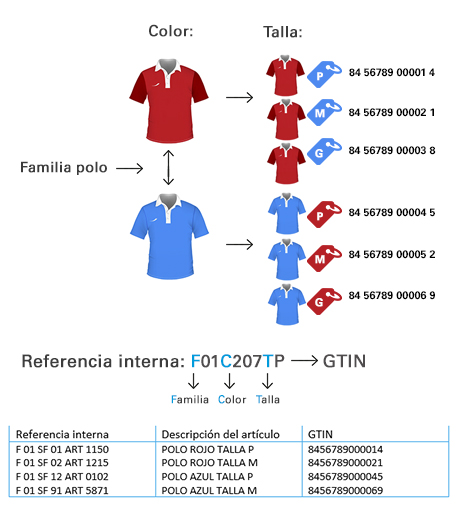
\includegraphics[scale=0.7]{./Capitulo2/figs/catalogo_post_barras.jpg}
  \caption{Referencia interna para la estructura de código de barras en la creación de catálogs de productos.}
  \label{catalogo_post_barras}
\end{figure}

\subsection{Codificaciones de agrupaciones}

Una agrupación es un conjunto de unidades de consumo cuya función es facilitar el manipulado de éstas, tanto en lo que se refiere a los envíos, como a los procesos de entrega, recepción, etc.\\

Todas las agrupaciones pueden ser separadas en las unidades de consumo que las forman.\\

Es correcto identificar una agrupación asignando un código GTIN-13 que identifique a la misma, distinto al de la unidad de consumo que contiene.\\

También es posible identificar la agrupación mediante un código GTIN-14. Éste se obtiene añadiendo delante del GTIN-13 de la unidad de consumo una Variable Logística.\

La variable logística es el dígito situado a la izquierda del código GTIN-14 de la unidad de consumo.\\

Los valores que puede tomar están entre el 1 y el 8, ambos inclusive. [\citep{CCCB:2019:Online}]

\begin{figure}
  \centering
    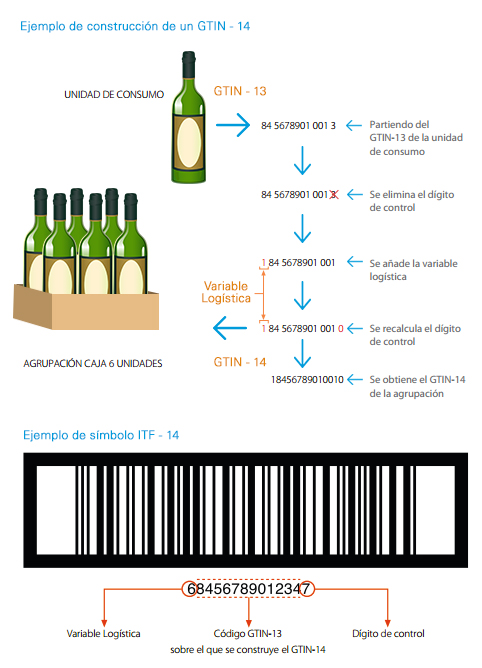
\includegraphics[scale=0.8]{./Capitulo2/figs/codificacion_agrupaciones_post_barras.jpg}
  \caption{La codificación de agrupaciones permite manipular un conjunto de unidades, que puede ser útil para su manipuleo y transporte.}
  \label{codificacion_agrupaciones_post_barras}
\end{figure}
           % ~20 páginas - Poner un contexto a la tesis, hacer referencia a trabajos actuales en el tema

%%%%%%%%%%%%%%%%%%%%%%%%%%%%%%%%%%%%%%%%%%%%%%%%%%%%%%%%%%%%%%%%%%%%%%%%%
%           Capítulo 3: Diseño e implemantacion                         %
%%%%%%%%%%%%%%%%%%%%%%%%%%%%%%%%%%%%%%%%%%%%%%%%%%%%%%%%%%%%%%%%%%%%%%%%%

\chapter{Diseño del experimento}

\\
El desarrollo de la aplicación considera las siguientes situaciones para considerar un sistema útil para el manejo de almacenes. Dentro de las características útiles se menciona los siguientes puntos.

\begin{enumerate}
\item Registro de usuario
\item Modificación de Almacenes
\item Modelamiento de productos
\end{enumerate}

Entre las características principales de un sistema de gestión de almacenes están los siguientes puntos.

\begin{enumerate}
\item Códigos de barras
\item Herramientas de informes
\item Previsión de inventarios
\item Alertas de inventarios
\end{enumerate}

%%%%%%%%%%%%%%%%%%%%%%%%%%%%%%%%%%%%%%%%%%%%%%%%%%%%%%%%%%%%%%%%%%%%%%%%%
%                          Modelamiento de Almacenes                    %
%%%%%%%%%%%%%%%%%%%%%%%%%%%%%%%%%%%%%%%%%%%%%%%%%%%%%%%%%%%%%%%%%%%%%%%%%
\section{Modelamiento de los almacenes}

\\
Dentro de un contexto variado de empresa, lo normal es dividirlas en dos grupos, que son empresas dedicadas a la fabricación y empresas dedicadas al comercio. De estos dos grupos de empresas, la gestión de almacenes es diferente. La gestión de almacenes en empresas dedicadas a la fabricación debe de considerarse un flujo interno que describa los movimientos de los materiales internamente para su transformación. Sin embargo tanto para la empresa dedicada a la fabricación de productos como a una empresa dedicada al comercio, ambos tienes que gestionar almacenes para la venta; en el caso de la primera esta gestión será para los productos terminados y una empresa comercial, le interesará la gestión de sus mercaderías a la venta.\\

En el siguiente listado se muestra un resumen de las necesidades para una empresa de fabricación y una dedicada al comercio. [\citep{PCD:2019:Online}]

\begin{enumerate}
\item PARA FABRICACIÓN
\begin{enumerate}
\item Seguimiento de materiales
\item Niveles de inventario para piezas y productos terminados
\item Re-ordenación automática
\item Integración ERP
\end{enumerate}
\item PARA ALMACENES
\begin{enumerate}
\item Sistema de códigos de barras avanzado (QR, y demás)
\item Soporte a ubicación múltiple
\item Sistema de seguimiento de estantería
\item Soporte de selección de pedidos
\end{enumerate}
\end{enumerate}

Cabe aclarar que el listado anterior no implica una necesidad en cada uno de los tipos de empresas ya que cada empresa puede prescindir de alguna de ellas, claro que esto también implicaría un costo asociado.

%%%%%%%%%%%%%%%%%%%%%%%%%%%%%%%%%%%%%%%%%%%%%%%%%%%%%%%%%%%%%%%%%%%%%%%%%
%                          Modelado                                     %
%%%%%%%%%%%%%%%%%%%%%%%%%%%%%%%%%%%%%%%%%%%%%%%%%%%%%%%%%%%%%%%%%%%%%%%%%
\section{Modelamiento de usuario}

El funcionamiento de sistemas en línea es el usuario el elemento por donde la aplicación funciona. Si bien no se está creando un sistema de gestión de usuarios, se debe modelar un correcto uso de recursos en función al usuario.\\

Un sistema en línea, debe proveer las opciones para que un usuario cualquiera pueda acceder a él. Para tal efecto es importante crear mecanismos de registro, con validación para que el usuario pueda registrarse y acceder a sus recursos.\\

El registro no debe ser complejo ni tomar mucho tiempo. Desde este punto de vista, el usuario debe registrar sus datos básicos, como ser su nombre y su correo electrónico. Estos datos son almacenado y además es importante que el usuario ingrese una clave de acceso, la que llamaremos “Password”. Muchos sistemas, realizan comprobaciones para que el “Password” de usuario sea lo más seguro, tanto para el usuario como para el sistema mismo.\\

De los detalles anteriores, se deriva los siguientes diagramas que modelan el usuario en el sistema.

\begin{figure}
  \centering
    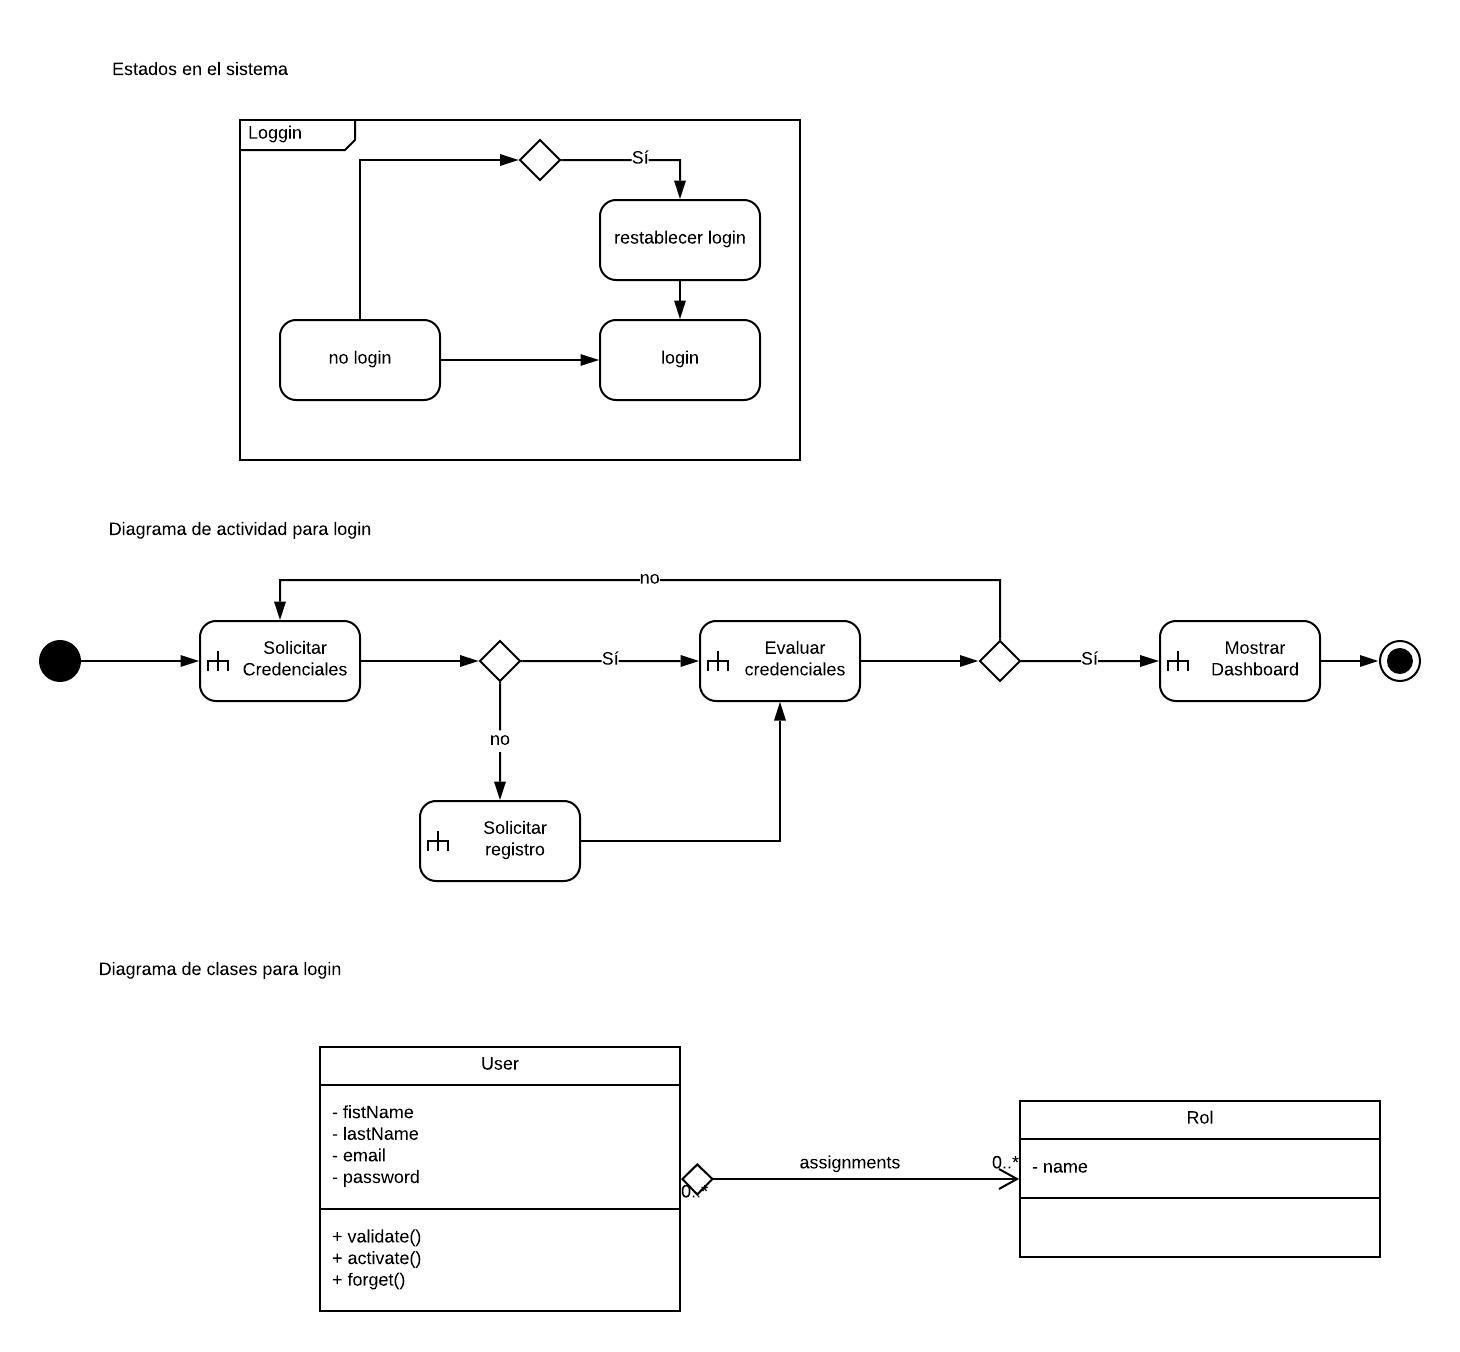
\includegraphics[scale=0.7]{./Capitulo3/figs/ADDStock-user-login.jpeg}
  \caption{Diagrama de estados, diagrama de actividades y diagrama de clases para el modelamiento de usuarios en el sistema de gestión de almacenes.}
  \label{user_login}
\end{figure}

El funcionamiento de manejo de usuarios en el sistema, se basa en el concepto de roles, lo cual permite al sistema manejar opciones. La división por roles nos permite definir accesos a diferentes opciones en el sistema. Para el propósito del sistema de gestión de almacenes, lo importante es permitir al usuario mismo, proteger su información de usuarios con menos privilegios que están encargados de tareas más concretas dentro de un sistema de almacenes.\\

La estructura de roles básicos que se puede manejar en el sistema son los siguientes:

\begin{itemize}
\item Superadmin
\item Admin
\item User
\begin{itemize}
\item Vendedor
\item Almacenero
\end{itemize}
\end{itemize}

El listado anterior muestra una estructura básica, ya que la idea es permitir al usuario crear más usuarios con roles que el mismo usuario pueda definir y por lo tanto los accesos que puedan tener a los recursos que vaya creando el usuario.\\

Se ha tomado pequeñas funciones que todos los sistemas de usuarios manejan y son la recuperación de “Password” de usuario y la mantención de sesión.

\subsection{La persistencia de la información}

En cuanto a la persistencia de la información, debe de realizarse ciertas consideraciones. Primeramente el motor de base de datos ideal será un sistema relacional, cabe considerar la existencia de motores no relacionales. En el mundo de motores relacionales esta los sistemas PostgreSQL, MySQL, Oracle, Microsoft SQL entre otros. Para los sistemas no relacionales tenemos los motores MongoDB, Redis, Elasticseach entre otros.

\begin{table}[htdp]
\centering
\begin{tabular}{||c | c | c ||}
\hline
\hline
\textbf{-} & \textbf{Database} & \textbf{Tipo} \\
\hline
\hline
1 & Oracle & Relational DBMS \\
\hline
\hline
2 & MySQL & Relational DBMS \\
\hline
\hline
3 & Microsoft SQL Server & Relational DBMS \\
\hline
\hline
4 & PostgreSQL & Relational DBMS \\
\hline
\hline
5 & MongoDB & Document store \\
\hline
\hline
6 & IBM Db2 & Relational DBMS \\
\hline
\hline
7 & Redis & Key-value store \\
\hline
\hline
8 & Elasticsearch & Search engine \\
\hline
\hline
9 & Microsoft Access & Relational DBMS \\
\hline
\hline
10 & SQLite & Relational DBMS \\
\hline
\hline
\end{tabular}
\caption[Para el mes de enero de 2019`]{Los 10 motores de bases de datos más populares. \\ Fuente https://fyaromo.com.co/2019/01/30/los-motores-de-bases-de-datos-mas-populares-relacionales-y-nosql/}
\label{tab:tabla-db-list} 
\end{table}
Fuente https://fyaromo.com.co/2019/01/30/los-motores-de-bases-de-datos-mas-populares-relacionales-y-nosql/

El objetivo de esta sección es poder seleccionar un motor de base de datos que puede trabajar de la mejor manera y permita un mejor desempeño y un mejor manejo de los datos. Por lo tanto, entre las características necesarias del sistema están listadas a continuación.

\begin{itemize}
\item Gran capacidad de almacenamiento.
\item Extensibilidad.
\item Escalabilidad.
\item Seguridad.
\item Optimizado para la búsqueda.
\item Resistencia ante los fallos.
\end{itemize}

Como puede observase en la Tabla \ref{tab:tabla-db-list}, esta tabulada mediante sus propiedades de ser un motor de base de datos relacional o no. Aunque no define ninguno de los atributos mencionados en la lista anterior. 

\section{Modelamiento de la empresa}

El sistema define la existencia de una empresa con cada cuenta de usuario. De este modo, se tiene una restricción de una empresa por cuenta creada. Sin embargo cada empresa puede tener definido varios usuarios, por lo cual haremos uso de los roles para definir una cuenta principal, que estará a cargo de la empresa y de los usuarios de esta misma.\\

El modelamiento general estará basado en una sola clase, que manejará la información de la empresa.\\

\begin{figure}
  \centering
    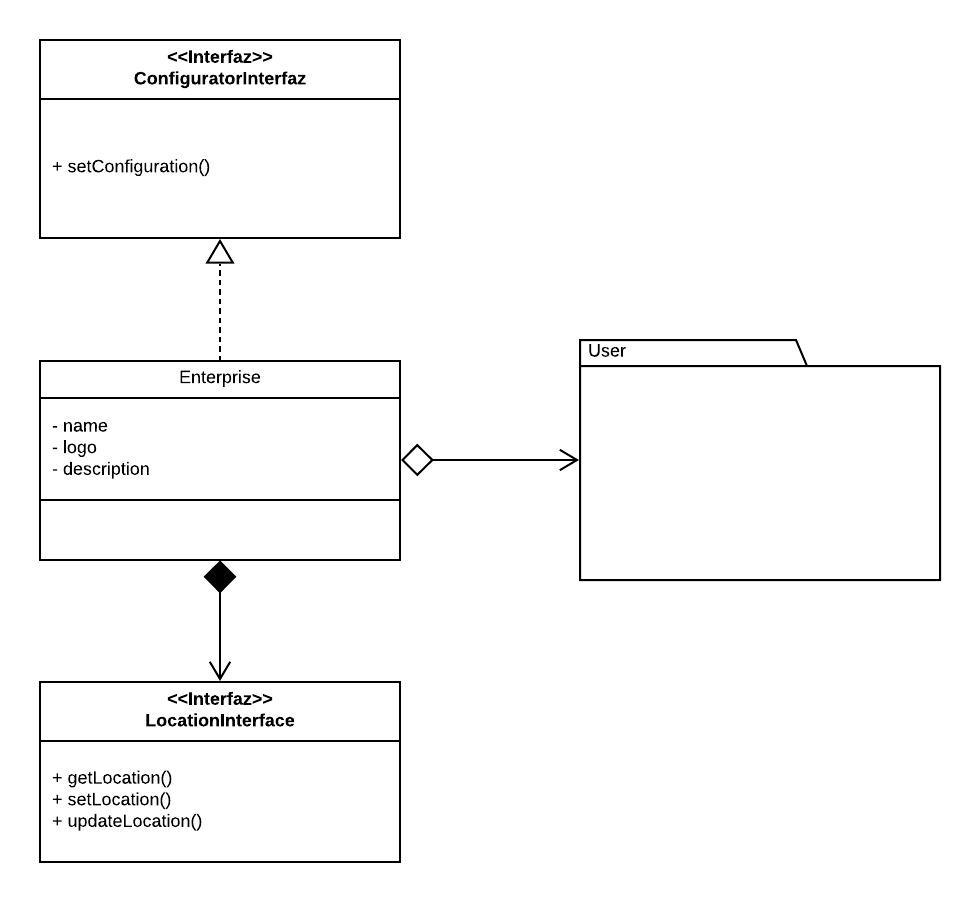
\includegraphics[scale=0.9]{./Capitulo3/figs/ADDStock-enterprise.jpeg}
  \caption{Diagrama de clases para el modelamiento de empresa.}
  \label{enterprise}
\end{figure}

La definición de empresa se basa en la información que se requiere guardar y esencialmente se trata del nombre de la empresa y su dirección. Cabe mencionar que la información tiene que ser guardada y está íntimamente ligada a las configuraciones que haya a realizarse en la aplicación.\\

En el modelo (figura \ref{enterprise}) presentado se trata de especificar que la clase empresa interviene en las configuraciones que se realizarán en la aplicación. Mediante el objeto empresa se realizará las configuraciones en la aplicación.\\

Este modelo mostrado en \ref{enterprise} requiere una explicación de porqué se está usando una \textbf{interface} para la localización. La idea general de localización está muy ligada a los almacenes, ya que se puede definir sucursales, puntos de donde los proveedores se encuentren y varios productos pueden estar en distintos lugares para su almacenado.

La información que será necesaria almacenar esta representada en el diagrama \ref{ER-diagram-v1}.

\section{Modelando el producto}

El producto es el tema principal de la aplicación y la información circulara en función a los productos que se tengan almacenados o en proceso. Incluso los productos que sean considerados de distinta manera, como por ejemplo los materiales, suministros, estos a su vez pueden tener un grado más de especialización ya que pueden ser materiales de transformación, materiales de uso como son los consumibles.\\

En este modelamiento todavía no se tomará en cuenta los movimientos de productos en almacenes ni su almacenamiento propiamente dicho.\\

La necesidad de información que hasta ahora se ha modelado corresponde a la figura \ref{Product-classes}

\begin{figure}
  \centering
    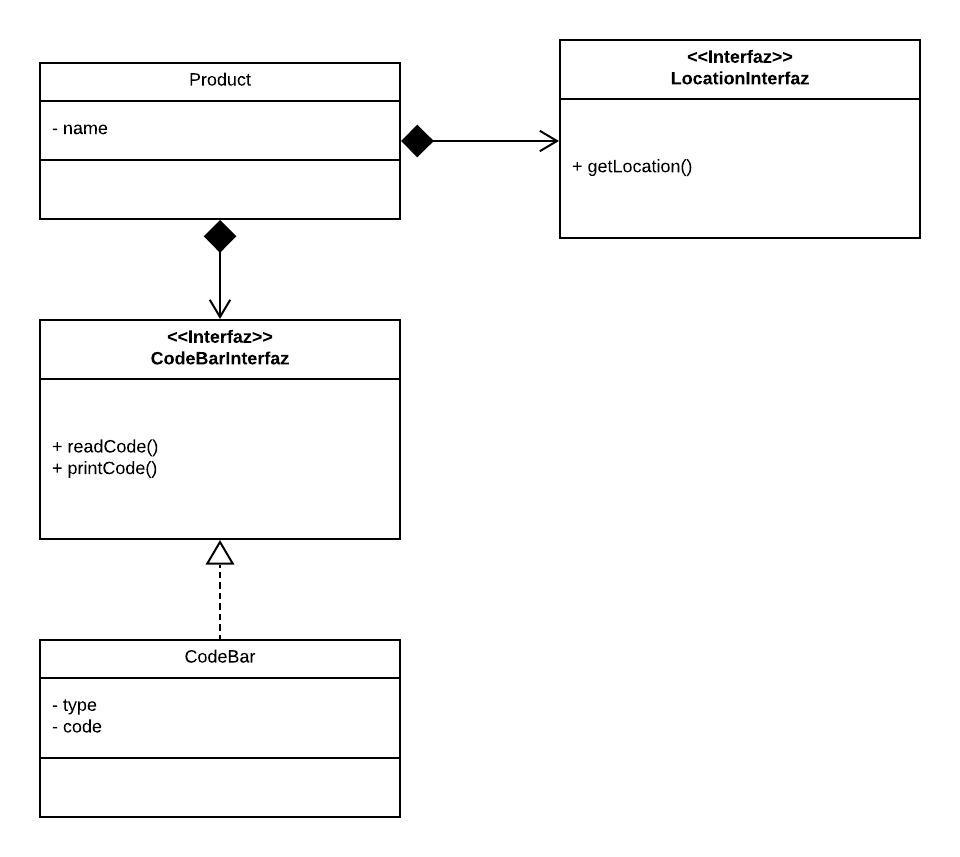
\includegraphics[scale=0.9]{./Capitulo3/figs/ADDStock-Product.jpeg}
  \caption{Diagrama de clases para el modelamiento de producto.}
  \label{Product-classes}
\end{figure}

La información general del producto viene dada por los valores de (name, description, price). Esta tupla de valores refleja la información de un producto que se podría manejar en una empresa.\\

Para el propósito del modelamiento y de la utilidad para la empresa en el manejo de un producto para almacenes es necesario considerar más valores. Para este propósito se elaboró una lista que describe a un producto.

\begin{itemize}
\item Nombre del producto.
\begin{itemize}
\item El producto puede ser vendido.
\item El producto puede ser comprado.
\end{itemize}
\item Tipo del producto.
\item Categoría.
\item Referencia interna. (Código o identificación interna)
\item Código de barras.
\item Notas internas.
\item Precio Venta. Considere las unidades de la moneda.
\item Costo.
\item Inventario. Información referida a lugar donde esta almacenado el producto, además de la ruta que sigue el producto dentro de la empresa.
\item Logística.
\begin{itemize}
\item Responsable. Este valor es un usuario del sistema que pertenece a la empresa.
\item Peso.
\item Volumen.
\item Plazo de entrega del cliente.
\end{itemize}
\item Descripción para pedidos de entrega
\item Descripción para Recepciones
\end{itemize}

\subsection{Operaciones}

Las operaciones que son útiles dentro una empresa en cuanto a los productos o materiales son los siguientes:

\begin{enumerate}
\item Transferencias.
\item Reposición.
\item Ajustes de inventario.
\item Desechar.
\item Ejecutar planificador.
\end{enumerate}

Las operaciones listadas anteriormente son básicas y están orientadas a realizar 1) movimientos dentro la empresa con el fin de que estén disponibles donde se los necesite y sean útiles. 2) Las reposiciones representan las reglas para mantener un número de productos disponibles dentro los almacenes. 3) El ajuste de inventario representa la actividad de contar las unidades físicas de cada producto que esta registrado en el sistema; por lo que representa un control vital. Suele efectuarse cada periodo de tiempo que la empresa vea necesario. 4) Desechar significa que el producto en si, tiene algún defecto, da{o, deterioro y que ya no puede ser usado, dentro del ciclo del procesos en la empresa. 5) Todo lo anterior tiene como objetivo mantener un control automático, en ese sentido el sistema procede a realizar los controles y las notificaciones que el usuario haya indicado.\\

Un punto también importante en un sistema de gestión de almacenes es la capacidad de ser configurable. Esto significa que dentro del sistema se tiene las opciones de cambiar ciertos valores que al usuario le interese y se adapte mejor a sus necesidades.\\

En este punto se detalla los siguientes valores como configurables:

\begin{itemize}
\item Unidades monetarias.
\item Unidades de peso y volumen.
\item Categorías de los productos.
\item formato de fecha y hora
\end{itemize}

Cabe aclarar que puede existir algún valor que el usuario necesita que sea configurable; para ello el uso del sistema permitirá identificar este requerimiento. Sin embargo esto escapa un poco del alcance de este proyecto. Eso es un tema de mantenimiento.

\subsection{Modelamiento de la información del Producto}

La sección anterior es una descripción de las necesidades de un sistema de almacenes para manejar los productos. En esta sección la idea principal es obtener los diagramas para identificar las clases que están involucradas y que permitirán el funcionamiento del sistema. En un primer nivel de formulación para una solución mediante un diagrama de clases se presenta en la figura \ref{Product-classes-v2}.

\begin{figure}
  \centering
    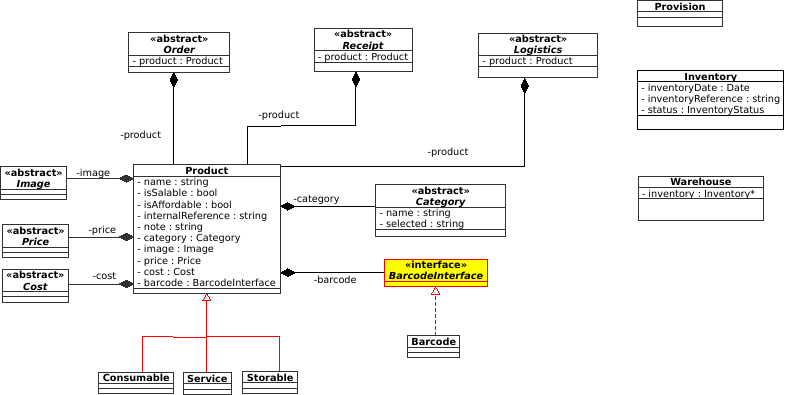
\includegraphics[scale=0.7]{./Capitulo3/figs/ADDStock-product-v2.png}
  \caption{Diagrama de clases para el modelamiento de producto en su segunda versión. En este diagrama se muestra las relaciones con los conceptos de Recepciones y Adquisiciones.}
  \label{Product-classes-v2}
\end{figure}

La idea general de esta propuesta de diseño (Figura \ref{Product-classes-v2}), se centra en la construcción de la clase \textit{Product}. El producto esta definido por atributos de clases y además tiene dependencias de las clases: \textit{Image}, \textit{Price}, \textit{Cost}, \textit{Category} y \textit{Bardcode}. Esta configuración trata de adaptar el patrón Builder, para lo cual se ha definido las dependencias de \textit{Product} como \textbf{asbtract} de esta manera sus clases concretas podrán ser manejadas por los métodos \textit{getProduct()} y \textit{buildPart()}. Los métodos mencionados anteriormente, son parte de la propuesta del patrón \textbf{Builder}. Este texto no tratará el patrón \textbf{Builder}, pero, se intentará explicarlo a lo largo del desarrollo de este capítulo.\\

Un segundo nivel de refinamiento se puede ver en la siguiente figura \ref{Product-classes-v3}.

\begin{figure}
  \centering
    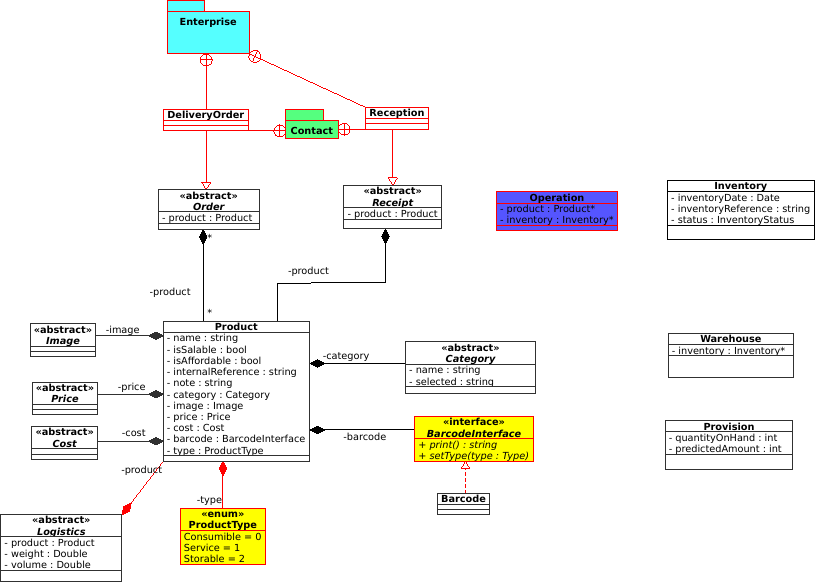
\includegraphics[scale=0.7]{./Capitulo3/figs/ADDStock-product-v3.png}
  \caption{Diagrama de clases para el modelamiento de producto en su tercera versión. En este diagrama se muestra las relaciones con las clases \textbf{abstract} y sus relaciones con otros módulos, como por ejemplo el módulo \textit{Enterprise}.}
  \label{Product-classes-v3}
\end{figure}

En la siguiente sección se desarrollará el diagrama de entidad-relación para el almacenamiento de los datos.

\section{Modelamiento Entidad-Relación}

Las secciones anteriores nos permite realizar un análisis de la interacción para generar un proceso. En el desarrollo del proceso, se genera información de forma de datos, que deben ser guardados.

Los datos generados en los procesos deben de guardarse, y para ello se modelará el sistema orientado a una base de datos relacional. Como se pudo observar en la tabla \ref{tab:tabla-db-list}, existe una variedad de motores de base de datos relacionales. Sin embargo, el sistema en desarrollo debe de escogerse un motor de base de datos que permita su funcionamiento.

La elección de una base de datos no es parte de este capítulo, por lo que nos centraremos en un modelamiento de base de datos en un alto nivel.

\begin{figure}
  \centering
    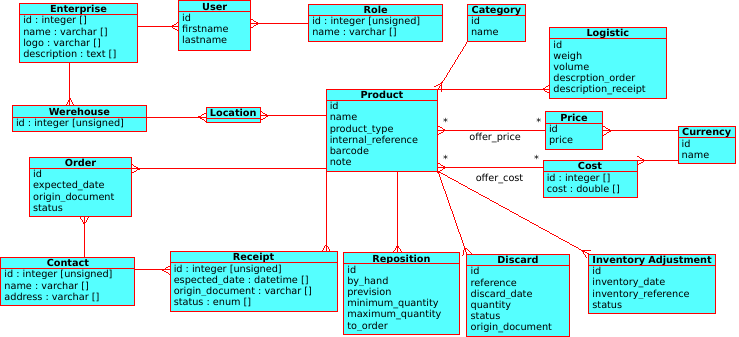
\includegraphics[scale=0.7]{./Capitulo3/figs/ADDStock-ER-diagram-v1.png}
  \caption{Diagrama Entidad-Relación. En este diagrama se muestra la relación que hay entre las distintas entidades que el sistema hará uso. La entidad que mas refleja relaciones es \textit{Product}. En esta entidad se ha tratado de establecer todos los atributos necesarios para su almacenaje en base de datos. Por otra parte cada entidad presenta ya un conjunto de atributos que se harán uso en el sistema.}
  \label{ER-diagram-v1}
\end{figure}

En el diagrama \ref{ER-diagram-v1}, se presenta una primera aproximación para el modelamiento de la información. Las entidades que se han podido definir en este diagrama son los siguientes:

\begin{itemize}
\item Category
\item Contact
\item Cost
\item Currency
\item Discard
\item Enterprise
\item Inventory\_Adjustment
\item Location
\item Logistic
\item Order
\item Price
\item Product
\item Receipt
\item Reposition
\item Role
\item User
\item Werehouse
\end{itemize}

Esta lista preliminar funcionará como punto de partida para hacer funcionar una primera versión del sistema de almacenes. Por lo tanto, el código que se generará de este diagrama, podrá ser subido a un motor de base de datos. Esta tarea se mostrará en el siguiente capítulo.
      % ~20 páginas - Explicar el problema en específico que se va a resolver, la metodología y experimentos/métodos utilizados
\chapter{DESARROLLO DEL PROYECTO}
\section{PROTOTIPO}
   % ~20 páginas - Presentar los resultados tal cual son, y analizarlos.
\chapter{Conclusiones}
\blindtext            % ~5 páginas - Resumir lo que se hizo y lo que no y comentar trabajos futuros sobre el tema

%%%%%%%%%%%%%%%%%%%%%%%%%%%%%%%%%%%%%%%%%%%%%%%%%%%%%
%                   APÉNDICES                       %
%%%%%%%%%%%%%%%%%%%%%%%%%%%%%%%%%%%%%%%%%%%%%%%%%%%%%
\appendix
% this file is called up by thesis.tex
% content in this file will be fed into the main document
\chapter{Código/Manuales/Publicaciones}
% top level followed by section, subsection

\section{Apéndice}

Apéndice
               % Colocar los circuitos, manuales, código fuente, pruebas de teoremas, etc.

%%%%%%%%%%%%%%%%%%%%%%%%%%%%%%%%%%%%%%%%%%%%%%%%%%%%%
%                   REFERENCIAS                     %
%%%%%%%%%%%%%%%%%%%%%%%%%%%%%%%%%%%%%%%%%%%%%%%%%%%%%
% existen varios estilos de bilbiografía, pueden cambiarlos a placer
\bibliographystyle{apalike} % otros estilos pueden ser abbrv, acm, alpha, apalike, ieeetr, plain, siam, unsrt

%El formato trae otros estilos, o pueden agregar uno que les guste:
%\bibliographystyle{Latex/Classes/PhDbiblio-case} % title forced lower case
%\bibliographystyle{Latex/Classes/PhDbiblio-bold} % title as in bibtex but bold
%\bibliographystyle{Latex/Classes/PhDbiblio-url} % bold + www link if provided
%\bibliographystyle{Latex/Classes/jmb} % calls style file jmb.bst

\bibliography{Bibliografia/referencias}             % Archivo .bib


\end{document}
